\begin{figure}[t!]
    \begin{minipage}{\textwidth}
        \begin{minipage}[b]{0.46\textwidth}
            \centering
            \resizebox{\linewidth}{!}
            {
            \begin{tabular}{lccccccc} 
                \toprule
                \textsc{Model / Architecture} & \textsc{Params.} & \textsc{Final ppl.} $\downarrow$ \\
                \midrule
                Transformer \hspace{10.2pt} (\colorbox{Main}{T9}) & 29M & 2.769 \\[3pt]
                Mamba-2 \hspace{19.7pt} (\colorbox{Main}{M10}) & 33M & 2.757 \\[3pt]
                \model{} \hspace{-1.2pt} (\colorbox{EncDec0}{M3T1}+\colorbox{Main}{T15}+\colorbox{EncDec0}{M4}) & 64M & 2.705 \\[3pt]
                \model{} (\colorbox{EncDec0}{M3T1}+\colorbox{Main}{M15}+\colorbox{EncDec0}{M4}) & 66M & 2.697 \\
                \bottomrule
            \end{tabular}
            }
            \captionof{table}{\textbf{Model details and final performance on HG38.} We trained two isotropic models and two \model{} models, varying the main network architecture (Transformer or Mamba-2). Each \model{} model outperforms the corresponding isotropic model. We empirically find that the $\mathcal{E}^0=$\colorbox{EncDec0}{M3T1} encoder architecture slightly outperforms a pure Mamba-2 encoder $\mathcal{E}^0=$\colorbox{EncDec0}{M4} (\cref{sec: dna_supp}).
            }
            \label{tab: dna}
        \end{minipage}
    \hfill
        \begin{minipage}[b]{0.50\textwidth}
            \centering
            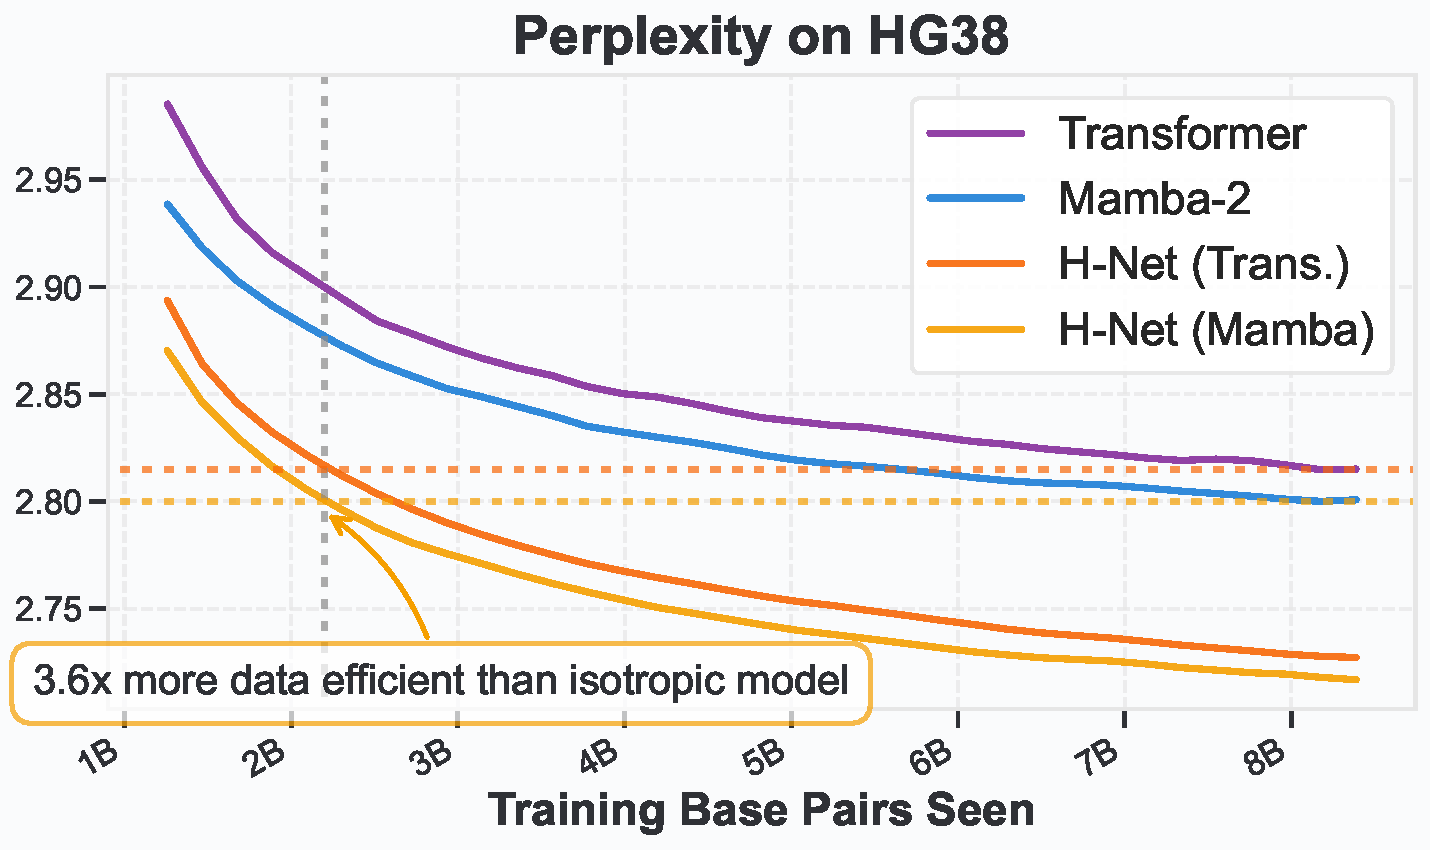
\includegraphics[width=\linewidth]{fig_img/dna.pdf} 
            \captionof{figure}{\textbf{Scaling performance on HG38} during the stable phase of training.
            Each \model{} model achieves the same pre-decay perplexity of the corresponding isotropic model with approximately $3.6\times$ less data. 
            }
            \label{fig: dna}
        \end{minipage}
    \end{minipage}
\end{figure}

